\begin{frame}
\huge
\begin{center}
BACKUP
\end{center}
\end{frame}

\begin{frame}\frametitle{Cosmic Shower and Muon Decay}
\begin{figure}
\caption{Cosmic shower induced by scattering of the incident cosmics proton of an air molecule. Charged and neutron pions are born in the reaction and then they further decay as $\pi^0 \rightarrow \gamma\gamma$, $\pi^+ \rightarrow \mu^+ + \nu_\mu$, $\pi^- \rightarrow \mu^- + \bar{\nu_\mu}$. Muon decay (to electron, neutrino and antineutrino through W-boson}
\label{fig:cosmicMuons}
\centering
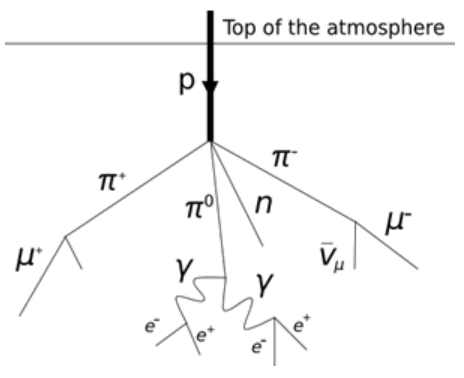
\includegraphics[width=0.35\textwidth, keepaspectratio=true]{figs/cosmicMuons.png}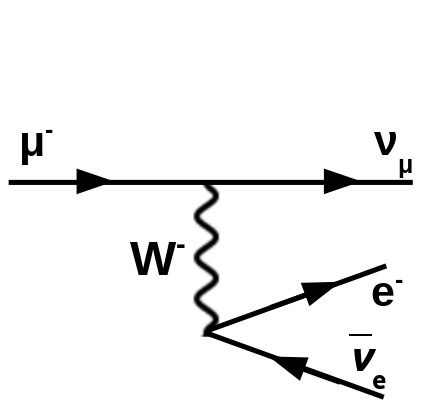
\includegraphics[width=0.35\textwidth, keepaspectratio=true]{figs/MuonDecay.png}
\end{figure}
\end{frame}

\begin{frame}\frametitle{$\nu$ oscillations probability with L/E}
\begin{figure}
\centering
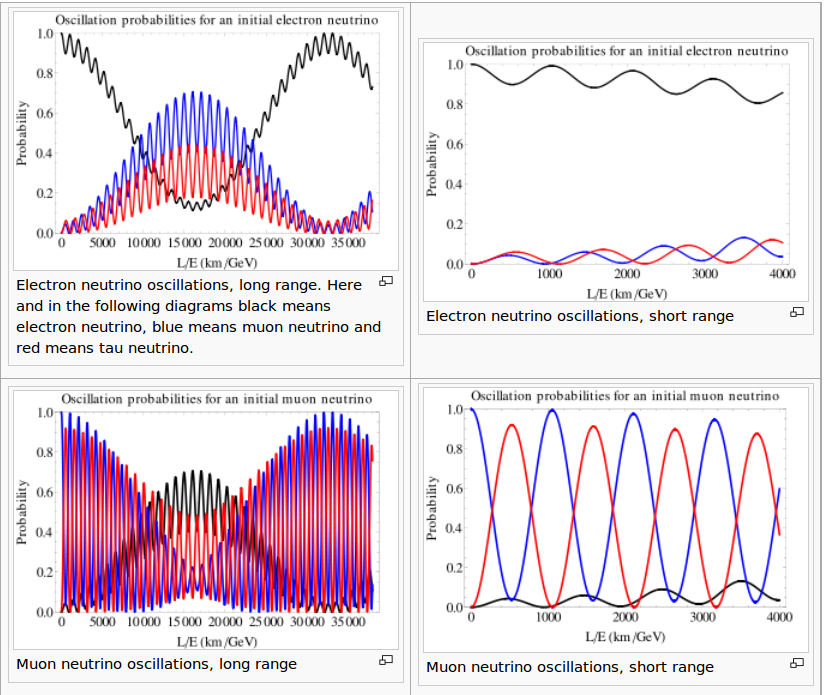
\includegraphics[width=0.80\textwidth, keepaspectratio=true]{figs/oscProbability_with_LtoE.png}
\end{figure}
\tiny
Source of figure: \cite{ref_fig_oscProbability_with_LtoE}
\end{frame}

\begin{frame}\frametitle{Solar $\nu$ spectrum and L/E}
\begin{figure}
\centering
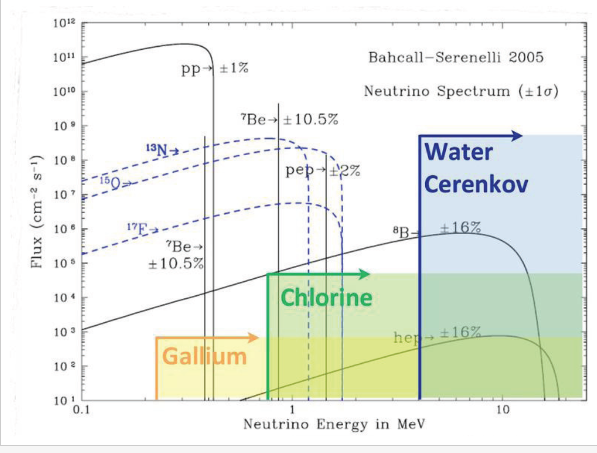
\includegraphics[width=0.70\textwidth, keepaspectratio=true]{figs/solarNeutrinoSpectrum.png}
\end{figure}
\scriptsize
$E~\sim~5~MeV~=~5\cdot10^{-3}~GeV$, $L~\sim~149.6 \cdot 10^6 km$, $\rightarrow$ $L/E~\sim~30\cdot 10^9 km/GeV$\\
$\Delta{E}~\sim~5~MeV$, $\Delta{L}~2000km+13000km=15000km$, $\Delta{L/E}~\sim~(L/E)^2 \cdot (\Delta{E}/E)^2~\sim~15~\cdot~10^9~km/GeV$\\
while oscillation period is $\sim~30~\cdot~10^3~km/GeV$\\
\tiny
Source of figure: \cite{ref_fig_solarNeutrinoSpectrum}
\end{frame}

\begin{frame}\frametitle{Theory. Two Neutrinos Case}
  \scriptsize
  \begin{center}
  $\nu_1=\nu_{\mu}cos\theta-\nu_esin\theta$\\
  $\nu_2=\nu_{\mu}sin\theta+\nu_ecos\theta$\\
  \end{center}
  \begin{center}
  $\nu_1(t)=\nu_1(0)e^{\frac{-iE_1t}{\hbar}}$, $\nu_2(t)=\nu_2(0)e^{\frac{-iE_2t}{\hbar}}$ $\leftarrow$ from quantum mechanics\\
  \end{center}
  Suppose, at t=0 there were $\nu_e(0)=1$, $\nu_\mu(0)=0$\\
  Then: $\nu_1(0)=-sin\theta$, $\nu_2(0)=cos\theta$, $\nu_1(t)=-{sin\theta}e^{\frac{-iE_1t}{\hbar}}$, $\nu_2(t)=-{cos\theta}e^{\frac{-iE_2t}{\hbar}}$\\
  Therefore, we are getting the system:\\
  \begin{center}
  $-{sin\theta}e^{-{{iE_1t} \over \hbar}}=\nu_\mu(t)cos\theta-\nu_e(t)sin\theta$,\\
  $-{sin\theta}e^{-{{iE_2t} \over \hbar}}=\nu_\mu(t)sin\theta-\nu_e(t)cos\theta$\\
  \end{center}
  By solving this system for $\nu_e$ and $\nu_\mu$, one would get:\\
  \begin{center}
  $P_{\nu_e \rightarrow \nu_\mu}=|\nu_\mu(t)|^2=[{sin2\theta}sin{\frac{(E_1-E_2)t}{2\hbar}}]^2$,\\
  $P_{\nu_e \rightarrow \nu_e}=|\nu_e(t)|^2=1-[{sin2\theta}sin{\frac{(E_1-E_2)t}{2\hbar}}]^2$\\
  \end{center}
\end{frame}

\begin{frame}\frametitle{Theory. Two Neutrinos Case}
  \scriptsize
  \begin{center}
  $P_{\nu_e \rightarrow \nu_\mu}=|\nu_\mu(t)|^2=[{sin2\theta}sin{\frac{(E_1-E_2)t}{2\hbar}}]^2$,\\
  $P_{\nu_e \rightarrow \nu_e}=|\nu_e(t)|^2=1-[{sin2\theta}sin{\frac{(E_1-E_2)t}{2\hbar}}]^2$\\
  \end{center}
  Therefore, for freely travelling neutrinos, if $\nu_e$ was emmitted, at any point there is a certain probability to register $\nu_e$ or $\nu_\mu$ and those probablities change with time periodically, by $~[sin(At)]^2$ law. That's why the phenomenon is called the neutrino oscillations.
  Suppose momenta $p_1=p_2$. Then using $E^2=p^2{\cdot}c^2+m^2{\cdot}c^4$ and assuming $m_{1,2}c^2 \ll E_{1,2}$: \\
  \begin{center}
  $P_{\nu_e \rightarrow \nu_\mu}=|\nu_\mu(t)|^2=[{sin2\theta}sin{\frac{(E_1-E_2)t}{2\hbar}}]^2=[{sin2\theta}sin{\frac{(m_1^2-m_2^2)c^3}{4\hbar{E}}z}]^2$\\  
  \end{center}
\end{frame}

\begin{frame}\frametitle{Theory. Three Neutrinos Case (continued)}
  \tiny
  The probability amplitudes of neutrino mixing are defined by parameters of the $U_{PMNS}$ but, analogous to simplified two-neutrino case described above, the differences of squares of neutrino masses also contribute to the probability. There are two independent expressionce for squares of masses differences: ${\Delta}m_{12}^2 = m_1^2-m_2^2$ and ${\Delta}m_{32}^2 = m_3^2-m_2^2$. Mass differences were measured in other neutrino oscillation experiments but the ${\Delta}m_{12}^2$ and ${\Delta}m_{32}^2$ present in the equations evenly and therefore the signs of these expressions were not measured. If the masses order as $m_3 > m_2 > m_1$, it's called normal neutrino mass hierarchy because other fundamental particles orders in a way that later generation particles have higher masses than lower generation particles. If the masses order as $m_1 > m_2 > m_3$ it's called inverted neutrino mass hierarchy. The mixing angles $\theta_{12}$, $\theta_{23}$, $\theta_{13}$ and differences of squared masses $|{\Delta}m_{12}^2|$ and $|{\Delta}m_{32}^2|$ are measured and give $U_{PMNS}$ matrix form of\\
  \begin{center}
  $|U_{PMNS}| \sim
  \begin{pmatrix}
  0.8 & 0.5 & 0.2 \\ 0.5 & 0.6 & 0.6 \\ 0.2 & 0.6 & 0.8 \\
  \end{pmatrix}$\\
  \end{center}
  The CP-violating phase $\delta_{CP}$ is unknown.\\
  The analogous matrix for quark mixing, Cabibbo-Kobayashi-Maskawa (CKM) matrix $V_{CKM}$, is much more diagonal:\\
  \begin{center}
  $|V_{CKM}| \sim
  \begin{pmatrix}
  1 & 0.2 & 0.004 \\ 0.2 & 1 & 0.04 \\ 0.008 & 0.04 & 1 \\
  \end{pmatrix}$\\
  \end{center}
  One of the important questions in modern particle physics is why the quark mixing angles are so much smaller than neutrino mixing angles and the other important question is whether there is any relationship between quark and neutrino mixing matrices.\\
\end{frame}

\begin{frame}\frametitle{About $U_{PMNS}$ Parametrization}
\begin{figure}
\centering
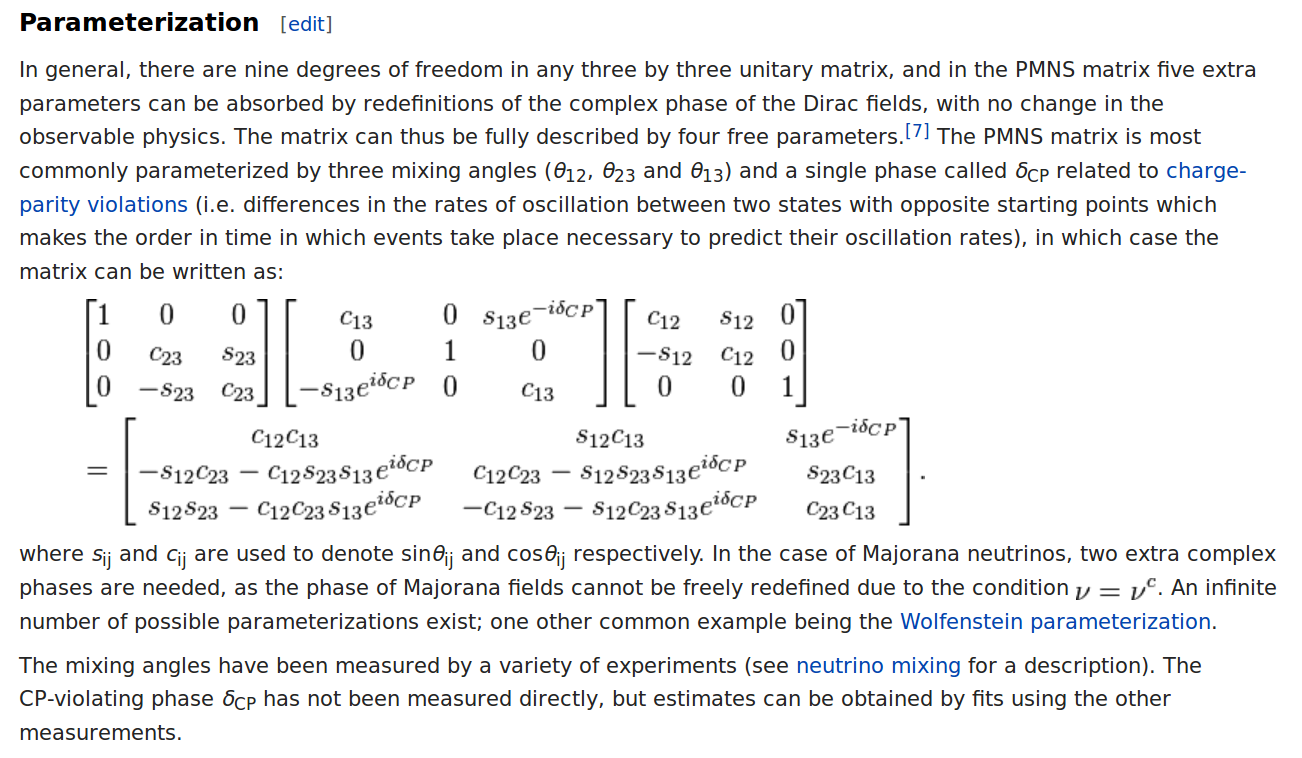
\includegraphics[width=0.90\textwidth, keepaspectratio=true]{figs/U_PMNS_parametrization.png}
\end{figure}
\tiny Source: \cite{ref_U_parametrization}
\end{frame}

\begin{frame}
\begin{figure}
\label{fig:LBNF_FermilabAccComplex}
\centering
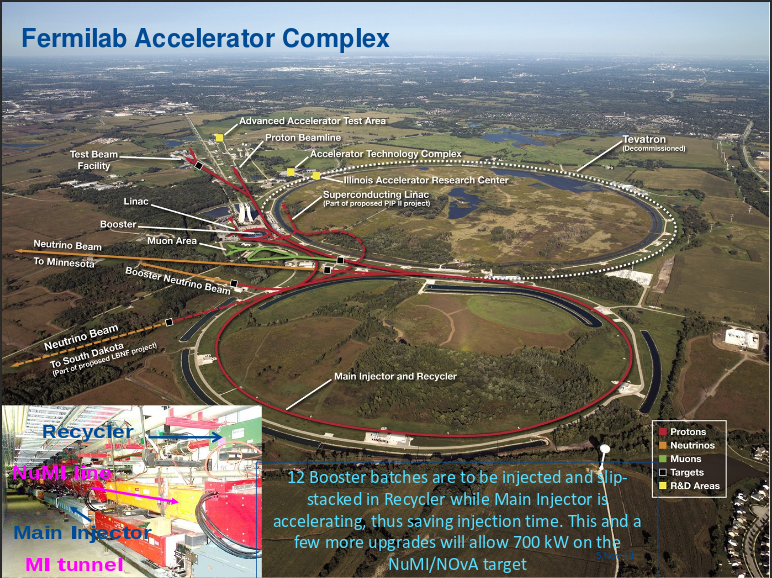
\includegraphics[width=0.95\textwidth, keepaspectratio=true]{figs/FermilabAccelerator.png}
\end{figure}
\end{frame}

\begin{frame}\frametitle{LBNF. Near Detector Physics}
\scriptsize
\begin{itemize}
  \item absolute flux measurement
  \item relative neutrino and antineutrino flux measurements
  \item flavor content of the neutrino source
  \item determination of the $E_\nu$-scale of neutrinos versus antineutrinos
  \item event-by-event measurements of NC interactions
  \item measurement of $\pi^0$, $\pi^\pm$, $K^\pm$, p, $K^0_S$ and $\Lambda$ in the NC and CC
%  \item "quasi-elastic and resonance measurements"
  \item nucleon structure, parton distribution functions and QCD studies
%  \item neutrino-argon interactions and nuclear effects
  \item precision measurements of electroweak physics
%  \item isospin physics and the Adler sum rule
%  \item measurement of the nuclean strangeness content
\end{itemize}
\end{frame}

\begin{frame}\frametitle{LBNF. Near Detector Physics, $\nu$ Oscillations}
\scriptsize
More specifically, the list of the physics measurements related to the neutrino oscillations to be performed by the Near Detector includes:
\begin{itemize}
  \item fluxes of $\nu_\mu$, $\bar{\nu_\mu}$, $\nu_e$ and $\bar{\nu_e}$. To distinguish between flavors, the measurement should rely on charged current interaction (fig. \ref{fig:MuonAndNeutronDecays}, middle and right) and measure the products of these interactions $\mu^-$, $\mu^+$, $e^-$, and $e^+$. (While the beam production system has the highest probability to produce muon neutrinos, the production of certain number electron neutrinos is also possible, for example, from charged kaon decays)
  \item $\nu_e$-$\bar{\nu_e}$ assymetries. For that, it's important not only distinguish between $\mu^\pm$ and $e^\pm$ but also between $e^-$ and $e^+$.
  \item the absolute $\nu_\mu$ and $\bar{\nu_\mu}$ fluxes need to be measured with $\simeq{3\%}$ precision in the neutrino energy range 0.5-8 GeV
  \item cross section of NC versus CC processes as a function of hadronic energy. NC is one of major backrounds which contribute to neutrino oscillation measurement
  \item yields of $\pi_0$ and photons. These particles are the most significant background to $\nu_e$ and $\bar{\nu_e}$ contamination
  \item fractions of the $\pi^\pm$ into the CC and the NC hadronic jets.    
\end{itemize} 
\end{frame}

\begin{frame}\frametitle{LBNF. Near Detector Targets (all)}
\begin{figure}
\centering
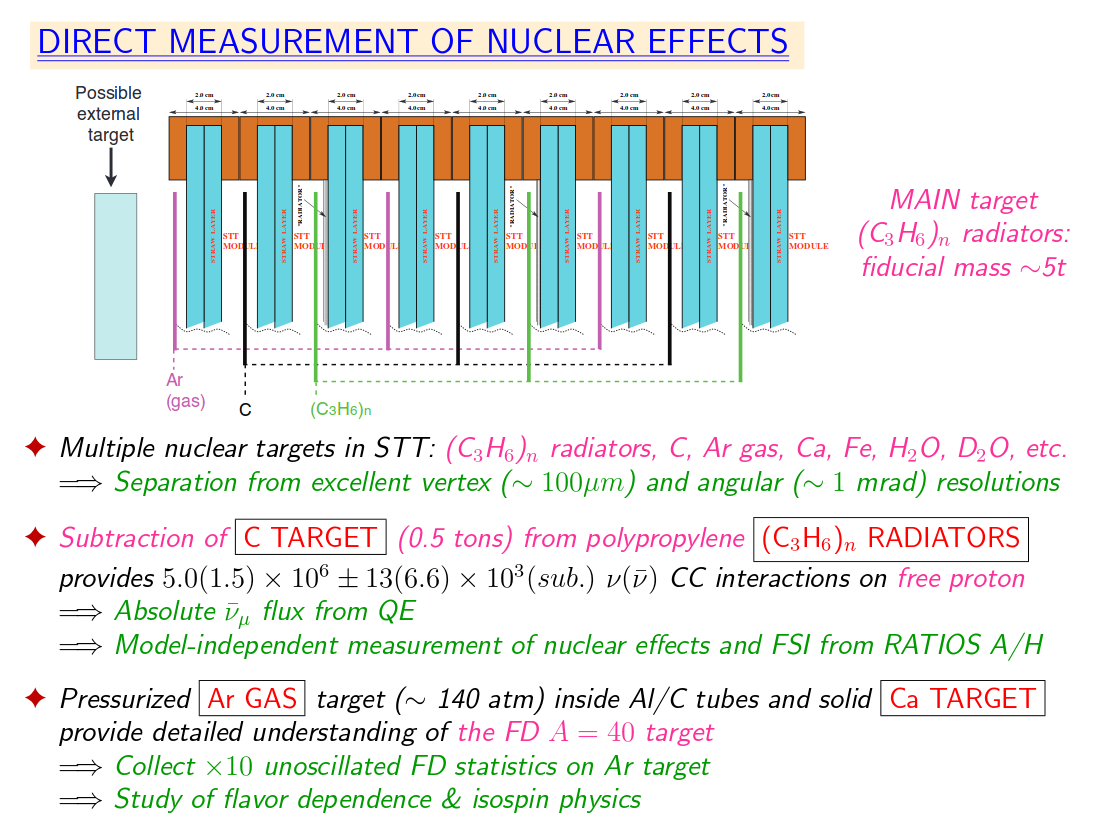
\includegraphics[width=0.80\textwidth, keepaspectratio=true]{figs/nearDetector_targets01.png}
\end{figure}
\tiny
Source of figure: presentation "Nuclear Targets and Precision Measurements in DUNE ND" by R. Petti at \cite{ref_LBNF_collaborationMeeting}
\end{frame}

\begin{frame}\frametitle{LBNF. Near Detector Targets (STT)}
\begin{figure}
\centering
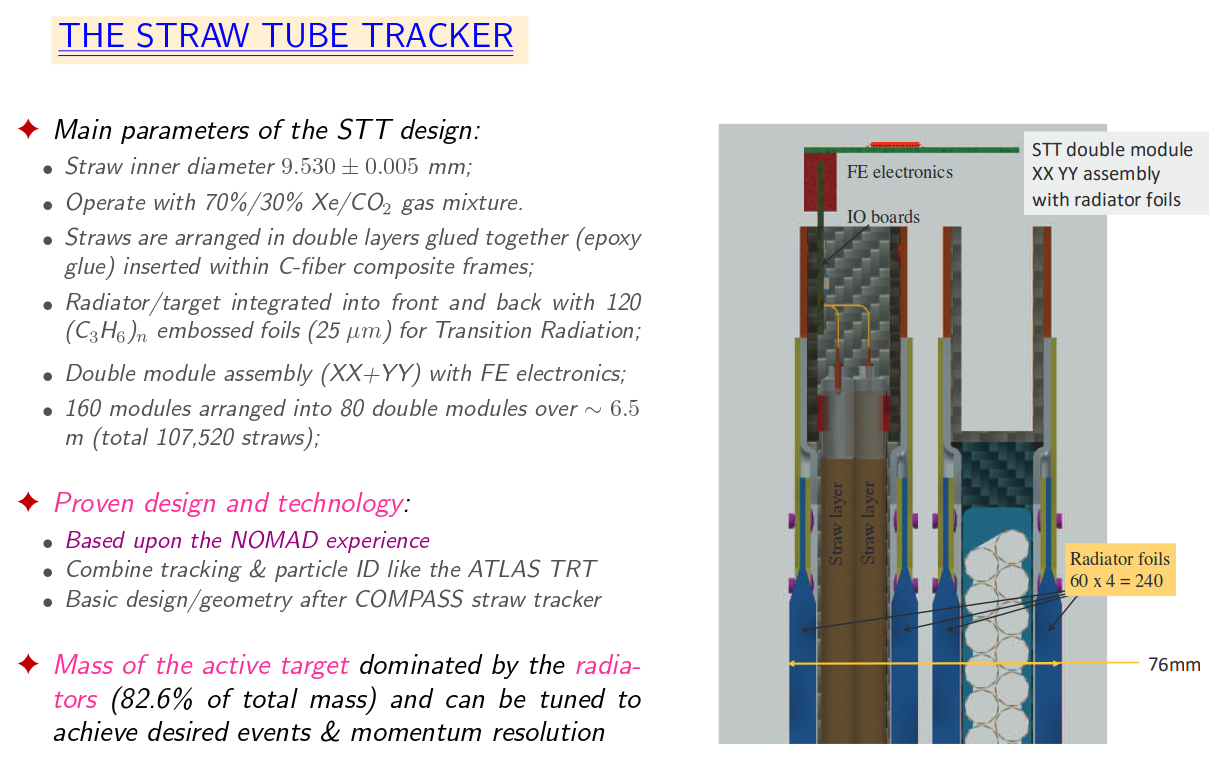
\includegraphics[width=0.80\textwidth, keepaspectratio=true]{figs/nearDetector_targets02.png}
\end{figure}
\tiny
Source of figure: presentation "Nuclear Targets and Precision Measurements in DUNE ND" by R. Petti at \cite{ref_LBNF_collaborationMeeting}
\end{frame}

\begin{frame}\frametitle{LBNF. Near Detector Targets Descriptions}
\begin{figure}
\centering
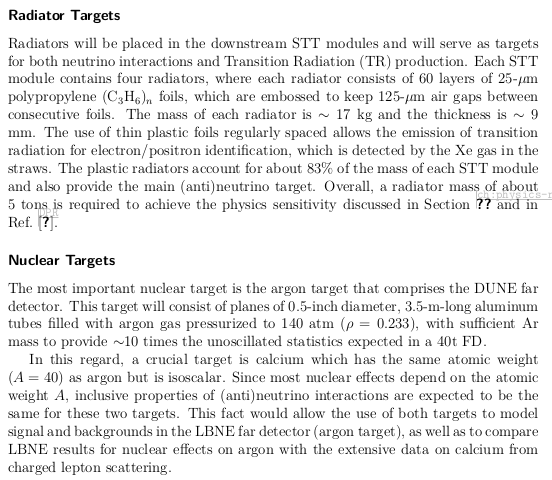
\includegraphics[width=0.80\textwidth, keepaspectratio=true]{figs/nearDetector_TargetsDescription.png}
\end{figure}
\tiny
Source of figure: \cite{ref_LBNFdoc_volume-detectors}
\end{frame}

\begin{frame}\frametitle{Mendeleev Periodic Table of Elements}
\begin{figure}
\centering
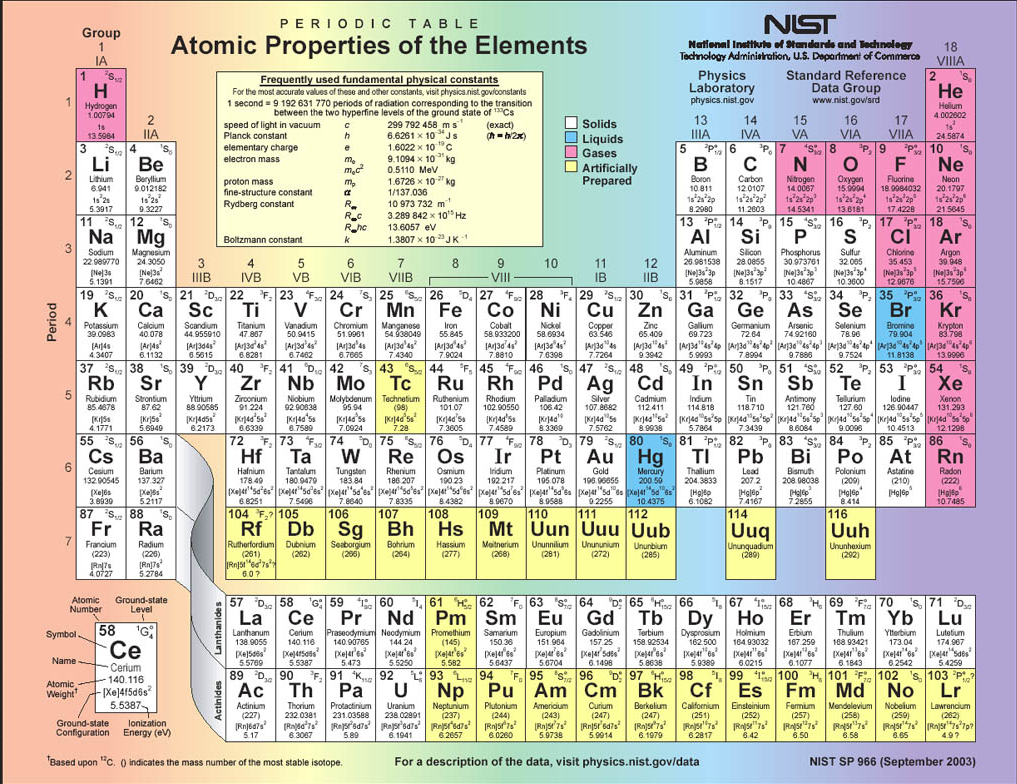
\includegraphics[width=0.90\textwidth, keepaspectratio=true]{figs/MendeleevTable.png}
\end{figure}
\tiny
Source of figure: \cite{ref_fig_MendeleevTable}
\end{frame}


